%%%% Paramétrage du TD %%%%
\def\xxactivite{Révisions \ifprof -- Corrigé \else \fi} % \normalsize \vspace{-.4cm}
\def\xxauteur{\textsl{Xavier Pessoles}}


\def\xxnumchapitre{Révision 1 \vspace{.2cm}}
\def\xxchapitre{\hspace{.12cm} Résolution des problèmes de statique -- Statique 3D}
\def\xxonglet{\textsf{Rév -- Stat}}
\def\xxactivite{\ifcolle Colle \else TD 02\fi }
\def\xxauteur{\textsl{Xavier Pessoles}}

\def\xxpied{%
Révision statique -- Résolution des problèmes de statique 3D\\
Fiche 1 -- \xxactivite%
}

\def\xxtitreexo{Quille pendulaire}
\def\xxsourceexo{\hspace{.2cm} \footnotesize{Concours Commun Mines Ponts 2014}}

\def\xxcompetences{%
\textsl{%
\textbf{Savoirs et compétences :}\\
\vspace{-.3cm}
\footnotesize
\begin{itemize}
\item \textit{Res1.C2.SF1} : Proposer une méthode permettant la détermination d’une inconnue de liaison.
\item \textit{Res1.C3.SF1} : Choisir une méthode pour déterminer la valeur des paramètres conduisant à des positions d'équilibre.
\item \textit{Res2.C18} : Principe fondamental de la statique.
\item \textit{Res2.C19} : Équilibre d’un solide, d’un ensemble de solides.
\item \textit{Res2.C20} : Théorème des actions réciproques.
\end{itemize}
\normalsize
}}

\def\xxauteur{\textsl{Xavier Pessoles}}


\def\xxfigures{
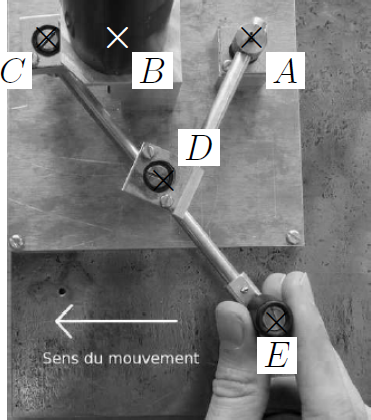
\includegraphics[width=.75\textwidth]{fig_00}
}%figues de la page de garde

\setcounter{exo}{0}
